\clearpage
\twocolumn[{%
\subsection{Noise and SNR}
\label{app:rq03_noise_and_snr}

\noindent\begin{minipage}[t]{0.485\textwidth}
\vspace{0pt}
\paragraph{Research Question.} \emph{How much does a measurement move when nothing but the seed or the checkpoint changes, how does that noise compare with the effect of a design decision, and what is each benchmark's signal-to-noise ratio under the 22 candidate definitions?}

\paragraph{Setup.} We use the deep cells with the baseline data that were trained with three seeds (175M and 600M at $K \in \{1, 2, 50\}$, 1B at $K \in \{1, 2, 30\}$). For each (size, $K$, task) cell, we divide the absolute effect of each design decision on the final score by a noise. The seed noise is the sample standard deviation across seeds. The checkpoint noise is the detrended standard deviation over the last 20\% of the run. Cells at chance are left out.
\end{minipage}\hfill
\begin{minipage}[t]{0.485\textwidth}
\vspace{0pt}
\begin{rqfinding}
\textbf{1. Seed noise exceeds checkpoint noise.} The seed std is a median 1.62$\times$ the detrended checkpoint std over 1467 ungated cells and larger in 74 \% of them (benchmarks 1.70 over 1310 cells, per-language BPB 1.33 over 139). Per size 1.60 at 175M, 1.77 at 600M and 1.56 at 1B. (Figure~\ref{fig:app_rq03_noise_and_snr}.)
\\
\\
\textbf{2. So the checkpoint-noise SNR is optimistic.} A design difference that clears the checkpoint noise need not clear a re-roll of the seed: on the same 1462 seed cells, depth's median effect is 2.07$\times$ the detrended checkpoint noise but 1.32$\times$ the seed noise (51 \% against 29 \% above 2$\times$).
\\
\\
\textbf{3. No design axis clears twice the seed noise in half of its cells.} Against seed noise the median effect is 1.32 for depth, 1.30 for scheme A vs B (540 cells, 29 \% above 2$\times$), 1.73 for scheme A vs C (195, 43 \%) and 1.53 for temperature T 1 vs 3 (1228, 38 \%).
\end{rqfinding}
\end{minipage}

\vspace{\baselineskip}
\noindent\begin{minipage}{\textwidth}
\centering
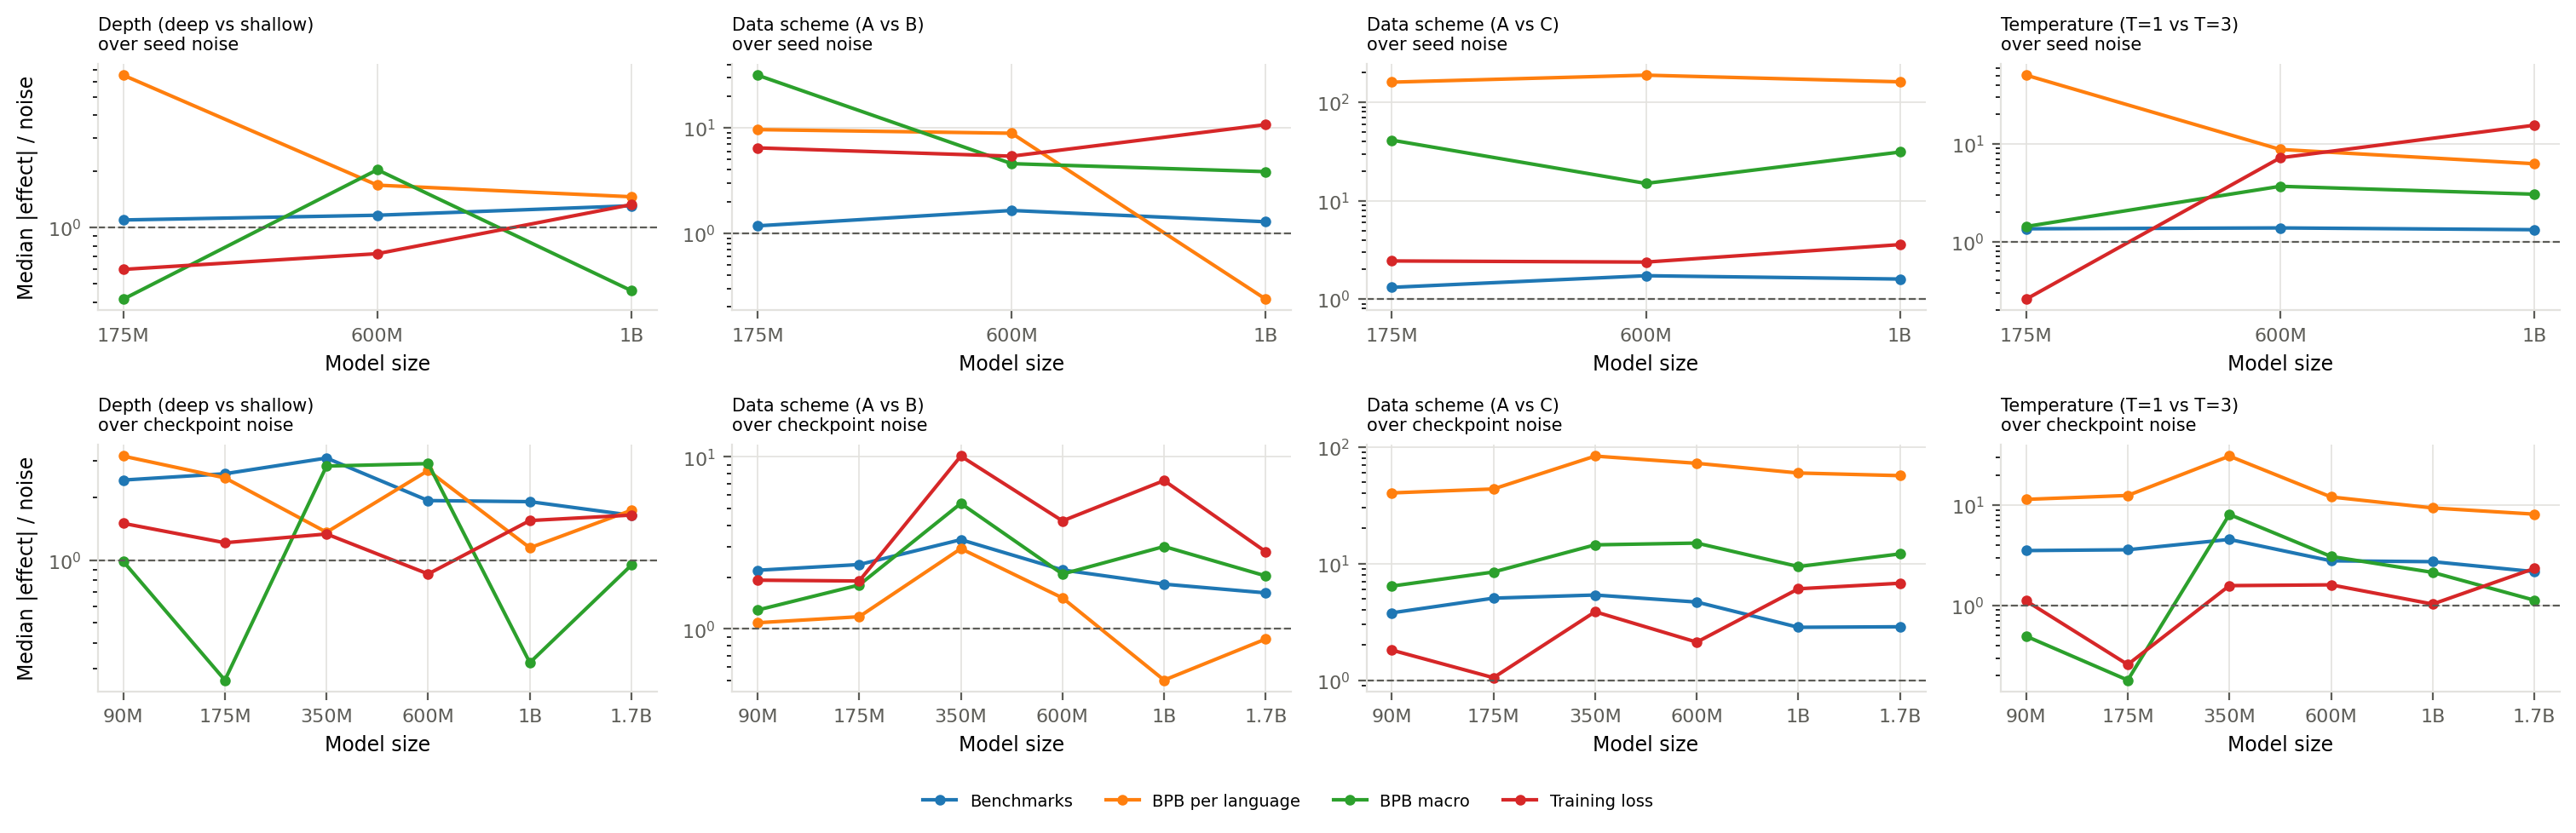
\includegraphics[width=\textwidth,height=0.4\textheight,keepaspectratio]{figures/app_rq03_noise_and_snr.png}
% source: src/signal-and-noise/analysis/rq03_noise_and_snr/pretraining/predictivity_seeds/effect_vs_noise_paper.png
\captionof{figure}{\textbf{Seed noise exceeds checkpoint noise.} Median absolute effect of each design decision over the noise, per model size, on the benchmarks, the per-language bits per byte, the macro average of the bits per byte and the training loss. Top row: over the seed noise. Bottom row: over the checkpoint noise. There is one column per decision. The dashed line at 1 is where the effect equals the noise (log scale).}
\label{fig:app_rq03_noise_and_snr}
\end{minipage}
\vspace{\baselineskip}
}]
